\icode{E-MG-CA-L3-261019-001}
已知某卫星在赤道上空的圆形轨道运行，卫星运动方向与地球自转方向相同，小明住在赤道上某城市，某时刻该卫星正处于小明的正上方，此后的一段时间里，小明观察到每三天恰好五次看到卫星掠过其正上方。已知地球的半径为\(R\)，自转周期为\(T_0\)，地球表面重力加速度为\(g\)，引力常量为\(G\)。求:
\begin{enumerate}
	\item 地球质量\(M\);
	\item 该卫星的轨道半径。
\end{enumerate}
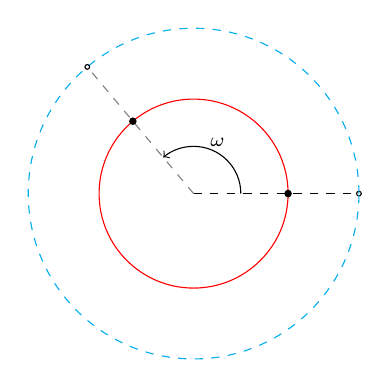
\begin{tikzpicture}[scale=.6,font=\scriptsize]
	\draw[red] (0,0) circle(2);
	\draw[dashed] (0,0)--(3.5,0);
	\fill (2,0) circle(.08);
	\draw (3.5,0) circle(.05);
	\draw[dashed,cyan] (0,0) circle(3.5);
	\draw[dashed,gray] (0,0)--(130:3.5);
	\fill (130:2) circle(.08);
	\draw (130:3.5) circle(.05);
	\draw[->] (1,0) arc (0:130:1);
	\node at(65:1.2) {\(\omega\)};
\end{tikzpicture}